\documentclass[10pt,twocolumn]{article}
\usepackage[letterpaper,margin=0.72in,columnsep=0.24in]{geometry}
\usepackage[T1]{fontenc}
\usepackage{newtxtext,newtxmath}
\usepackage{microtype}
\usepackage{graphicx}
\usepackage{booktabs}
\usepackage{tabularx}
\usepackage{array}
\usepackage{amsmath}
\usepackage{xcolor}
\usepackage{caption}
\usepackage{titlesec}
\usepackage{enumitem}
\usepackage[hidelinks]{hyperref}

\definecolor{navy}{HTML}{1F4E79}
\definecolor{teal}{HTML}{2A9D8F}
\definecolor{lightblue}{HTML}{EAF2F8}
\definecolor{lightgray}{HTML}{F2F4F7}

\captionsetup{font=small,labelfont=bf,skip=4pt}
\setlength{\parindent}{0pt}
\setlength{\parskip}{0.44em}
\setlist[itemize]{leftmargin=1.2em,itemsep=1pt,topsep=2pt}
\titleformat{\section}{\large\bfseries}{\thesection}{0.55em}{}
\titleformat{\subsection}{\normalsize\bfseries}{\thesubsection}{0.5em}{}
\titlespacing*{\section}{0pt}{1.0em}{0.35em}
\titlespacing*{\subsection}{0pt}{0.75em}{0.25em}
\renewcommand{\arraystretch}{1.08}

\begin{document}

\twocolumn[
\begin{@twocolumnfalse}
\begin{center}
{\fontsize{18}{21}\selectfont\bfseries
Domain-Balanced Uniform Adapter for Robust\\
Deepfake Detection under Sparse Local Degradation\par}
\vspace{0.45em}
{\normalsize Computer Vision Final Project, Track 2\par}
\vspace{0.28em}
{\small Final report, November 2026\par}
\end{center}

\vspace{0.35em}
\noindent\textbf{Abstract.}
Short-video deepfake detectors combine evidence from only a few face frames,
so changing which frames are degraded can change the final video decision.
We study this failure mode on the frozen GenD detector and train a small
residual adapter over its 1024-dimensional CLIP features. Our final method,
the Domain-Balanced Uniform Adapter (DBUA), samples real and fake videos from
Celeb-DF and DFDC in every batch and optimizes all six two-of-four blur masks.
On a fixed source-group Celeb-DF test split, DBUA raises degraded-condition
accuracy from 86.54\% for frozen GenD to 90.12\%, while improving clean
accuracy from 85.90\% to 91.03\%. A DFDC-only adapter transfers poorly to
Celeb-DF. Joint training recovers most of that loss but does not outperform a
Celeb-DF-only adapter. We therefore present the result as a data-composition
and negative-transfer study, not as evidence that adding data alone is a
methodological contribution. Paired source-group bootstrap intervals,
worst-mask accuracy, and explicit negative ablations are reported.

\vspace{0.5em}
\noindent\textbf{Keywords:} deepfake detection; local degradation; residual
adapter; domain generalization; robustness; GenD; Celeb-DF; DFDC
\vspace{0.8em}
\end{@twocolumnfalse}
]

\section{Introduction}

Deepfake detectors are commonly evaluated on clean frames, while online video
is blurred, compressed, resized, and mixed across heterogeneous capture
conditions. A video-level detector also has to combine a small set of frame
scores. These two properties interact: degrading only some frames can reverse
the aggregate decision even when the remaining frames still contain useful
evidence. We treat that position-dependent reversal as the central robustness
problem.

Prior studies show that preprocessing, quality degradation, and compression can
change detector behavior (Charitidis et al., 2020; Le \& Woo, 2023; Yang et
al., 2026). These failures
motivate an evaluation protocol that separates generic adaptation from
degradation-specific training.

The baseline is GenD, a published deepfake detector that operates on CLIP
ViT-L/14 visual features. We keep the 304M-parameter visual encoder frozen and
train a residual adapter over its cached features. This design makes repeated
mask experiments practical on one consumer GPU and isolates the effect of
adaptation from encoder fine-tuning (Yermakov et al., 2026).

The project asks three questions:
\begin{itemize}
  \item Does lightweight adaptation of frozen GenD features improve robustness
  to sparse local blur?
  \item Does mask-specific training add value beyond a clean-only adapter with
  the same trainable parameters and loss weight?
  \item Does training with a second dataset improve cross-dataset behavior, and
  what failure modes appear under domain shift?
\end{itemize}

The report separates these questions. It does not attribute every gain over
GenD to the mask objective, and it does not call additional data a new method.
The controlled comparisons, negative-transfer analysis, and failure cases are
part of the result.

\subsection{Related Work}

Deepfake detection research has developed from artifact-specific classifiers
toward models intended to transfer across datasets and generation methods.
GenD uses CLIP visual features and a compact classification head to improve
cross-benchmark behavior (Yermakov et al., 2026). Celeb-DF and DFDC provide
complementary evaluation settings: Celeb-DF emphasizes challenging synthesis
artifacts in celebrity videos, while DFDC contains a much larger and more
diverse collection of real and manipulated clips (Dolhansky et al., 2020; Li et
al., 2020).

A second line of work studies how preprocessing and low-level quality change
detector decisions. Compression, resizing, and blur can remove the traces
learned by a detector, and aggregation choices can change the final video score
(Charitidis et al., 2020). Quality-aware and degradation-consistent training
methods attempt to reduce this sensitivity by modeling quality conditions
explicitly (Le \& Woo, 2023; Yang et al., 2026).

Our study differs from global augmentation by changing only a sparse subset of
frame positions. This exposes the interaction between per-frame degradation and
video-level aggregation. We also separate target-domain adaptation from
zero-shot transfer, which is necessary for interpreting whether an additional
dataset improves robustness or only changes the calibration of the trained
head.

\begin{figure*}[t]
  \centering
  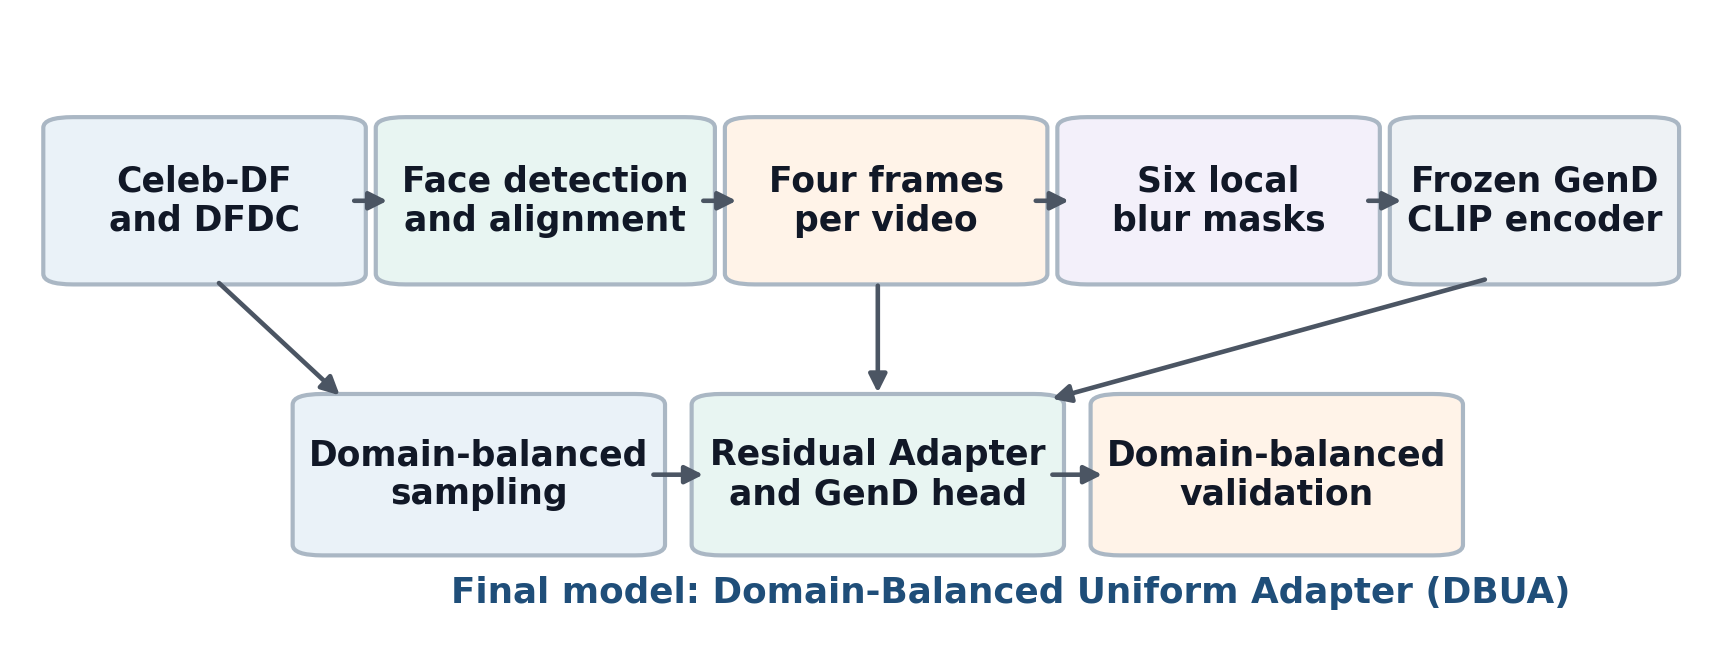
\includegraphics[width=0.96\textwidth]{figures_report_20261122/figure_1_pipeline.png}
  \caption{Training and evaluation pipeline. GenD remains frozen; the residual
  adapter is trained with domain-balanced samples and six local blur masks.}
  \label{fig:pipeline}
\end{figure*}

\section{Method}

\subsection{Residual feature adaptation}

For each of four aligned face frames, GenD produces an L2-normalized feature
vector $z\in\mathbb{R}^{1024}$. The residual adapter projects $z$ to a
64-dimensional bottleneck, applies GELU and dropout, projects back to 1024
dimensions, and combines the result with the original feature:
\begin{equation}
  h = \frac{z+\tanh(a)\,R(z)}
           {\left\lVert z+\tanh(a)\,R(z)\right\rVert_2},
\end{equation}
where $a$ is a learned scale initialized to zero and $R$ is the residual
branch. The original GenD two-class head is retained and updated with the
adapter. The trainable part contains approximately 0.13M parameters.

\subsection{Sparse local degradation}

We represent a video by four frame features. A binary four-position mask
selects which frames use blur features. The primary setting uses exactly two
blurred frames, giving six masks. Uniform training averages the video-level
binary cross-entropy over all six masks. This objective does not assume that a
particular frame position is more informative.

The training objective combines a clean-video loss and the mean masked loss:
\begin{equation}
  \mathcal{L}=0.5\,\mathcal{L}_{\mathrm{clean}}
  +1.0\,\mathcal{L}_{\mathrm{mask}}.
\end{equation}
The clean term preserves the original decision function, while the mask term
exposes the adapter to all frame positions. The final method excludes
prediction-consistency, feature-restoration, and identity penalties because
these variants produced weaker results.

\subsection{Domain-balanced sampling}

DBUA uses both Celeb-DF and DFDC during training. Each micro-batch contains 16
samples from each domain; within each domain, eight samples are real and eight
are fake. This addresses the DFDC class imbalance without discarding its
manipulation diversity. Validation keeps the two domains separate, computes a
class-balanced loss for each, and early-stops on their mean. The test splits
are never read during training or model selection.

\section{Experimental Protocol}

Celeb-DF and DFDC are partitioned by source group. For Celeb-DF, all videos
derived from the same identity pair remain in one split. For DFDC, a fake video
and the real source named by its \texttt{original} field remain in one split.
This prevents the same source from appearing in both training and test
partitions (Dolhansky et al., 2020; Li et al., 2020). Table~\ref{tab:data}
gives the resulting counts.

\begin{table}[t]
  \centering
  \caption{Fixed domain-aware split. Counts show videos; parentheses show
  real/fake videos.}
  \label{tab:data}
  \small
  \begin{tabular}{@{}lccc@{}}
    \toprule
    Domain & Train & Validation & Test \\
    \midrule
    Celeb-DF & 362 (124/238) & 78 (27/51) & 78 (27/51) \\
    DFDC part 0 & 934 (58/876) & 200 (16/184) & 200 (12/188) \\
    \bottomrule
  \end{tabular}
\end{table}

GenD and all adapters use the same face frames, degradation protocol,
classification threshold, and source-group partition. JPEG uses Pillow quality
30 with 4:2:0 subsampling. Resize uses bicubic downscaling to 25\% of width and
height. Blur uses a $9\times9$ Gaussian kernel. Four aligned $256\times256$
crops represent each video.

We report clean accuracy, mean local accuracy over six two-frame masks,
worst-mask accuracy, AUC, recovered and harmed mask events, and feature
similarity where relevant. Confidence intervals use 10,000 bootstrap resamples
over source groups. Masks are repeated measurements of the same videos and are
never treated as independent video samples.

\begin{table}[t]
  \centering
  \caption{Compared models and their roles.}
  \label{tab:models}
  \small
  \begin{tabular}{@{}p{0.22\columnwidth}p{0.31\columnwidth}p{0.34\columnwidth}@{}}
    \toprule
    Model & Training & Purpose \\
    \midrule
    Frozen GenD & None & Published baseline \\
    Celeb-DF-only & Celeb-DF train & Target-domain control \\
    DFDC-only & DFDC train & Zero-shot transfer test \\
    DBUA & Both train sets & Final model \\
    DBUA + identity & Both train sets & Regularization ablation \\
    \bottomrule
  \end{tabular}
\end{table}

\section{Results}

\subsection{Single-domain and dual-domain accuracy}

On the held-out Celeb-DF split, DBUA improves all four conditions over frozen
GenD. The target-domain-only adapter is still stronger, so the DFDC data do not
provide an independent gain on this target test.

\begin{table}[t]
  \centering
  \caption{Accuracy on the fixed Celeb-DF 78-video test split. The final column
  compares DBUA with the same-method Celeb-DF-only control.}
  \label{tab:single-dual}
  \small
  \begin{tabular}{@{}lcccc@{}}
    \toprule
    Condition & GenD & CDF-only & DBUA & DBUA-CDF \\
    \midrule
    Clean  & 85.90 & \textbf{93.59} & 91.03 & -2.56 \\
    Blur   & 83.12 & \textbf{90.38} & 88.82 & -1.57 \\
    JPEG   & 88.03 & \textbf{92.59} & 90.60 & -1.99 \\
    Resize & 88.46 & \textbf{91.31} & 90.95 & -0.36 \\
    \bottomrule
  \end{tabular}
\end{table}

\begin{figure*}[t]
  \centering
  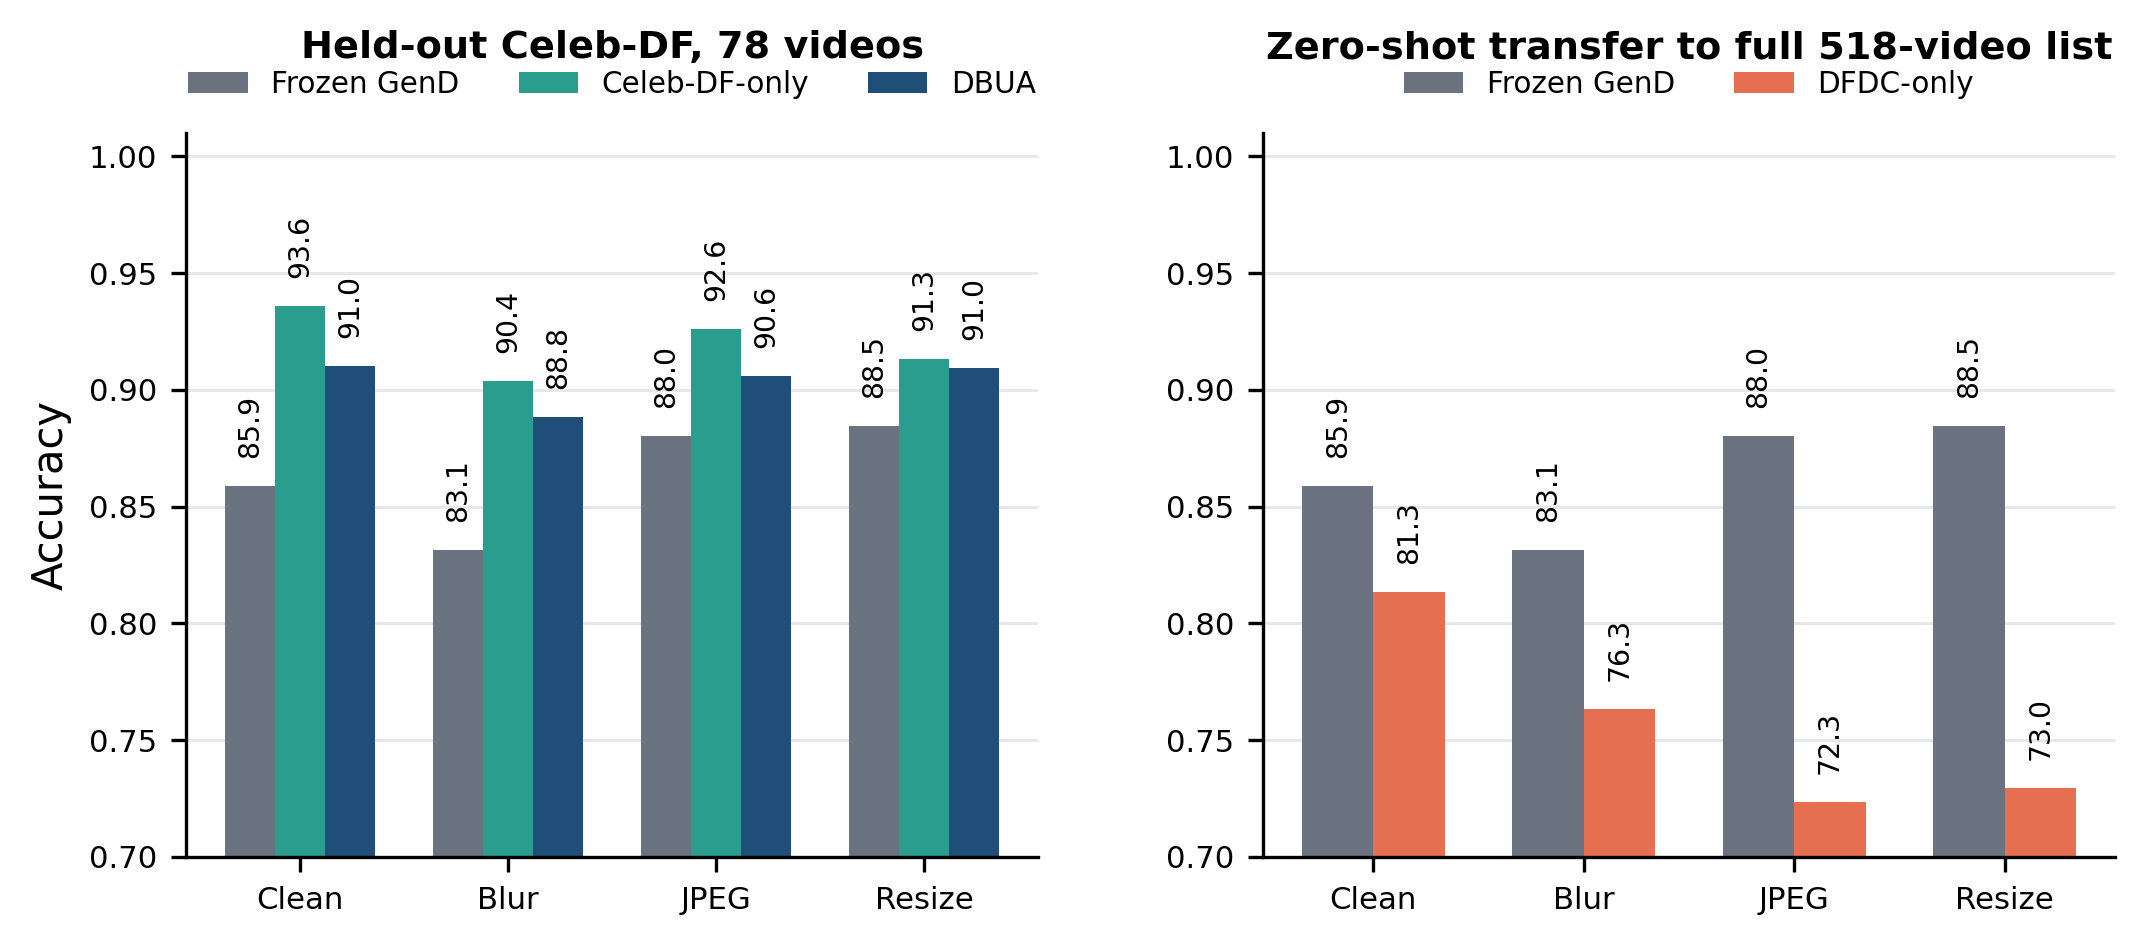
\includegraphics[width=0.94\textwidth]{figures_report_20261122/figure_2_domains.png}
  \caption{Left: the same 78-video Celeb-DF split separates the target-domain
  control from DBUA. Right: DFDC-only training causes clear negative transfer
  on the full 518-video list.}
  \label{fig:domains}
\end{figure*}

\subsection{Negative transfer from DFDC only}

DFDC-only adaptation learns its training domain well but does not transfer to
Celeb-DF. Relative to frozen GenD, clean accuracy falls from 85.90\% to 81.34\%.
Blur falls from 83.12\% to 76.33\%, JPEG from 88.03\% to 72.33\%, and resize
from 88.46\% to 72.95\%. The direction is not explained by a single threshold
because clean AUC also declines.

The likely cause is the combination of domain shift and a weak real-video
partition. DFDC part 0 contains only 86 real source groups, and the adapter
updates the final GenD head on features from a different face-crop and
generation distribution. The classification head moves away from the
calibration required by Celeb-DF even though training and validation losses
improve.

\subsection{Joint training and uncertainty}

DBUA recovers the DFDC-only loss and improves over GenD, but the bootstrap
intervals are wide. The Celeb-DF test split contains 78 videos and 52 source
groups, so each resample can move several percentage points. The intervals
describe source-group uncertainty and should not be interpreted as confidence
intervals over independent masks.

\begin{figure*}[t]
  \centering
  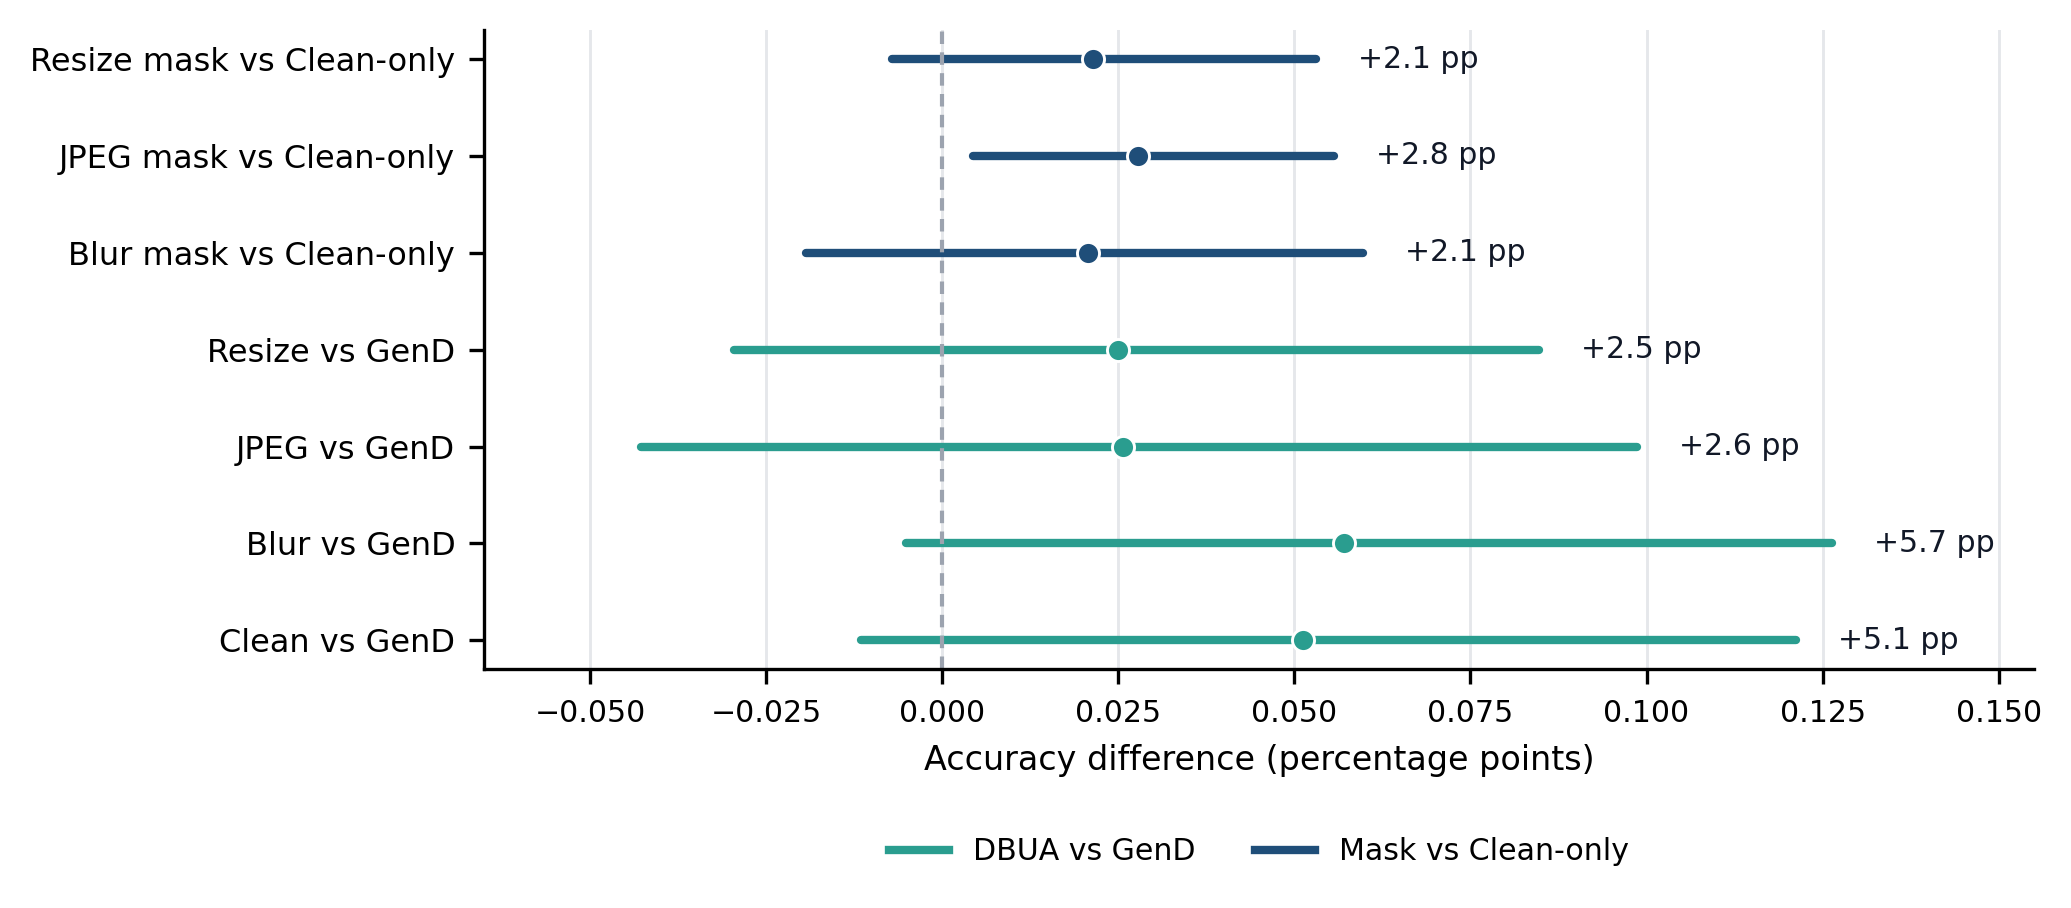
\includegraphics[width=0.93\textwidth]{figures_report_20261122/figure_3_ci.png}
  \caption{Paired source-group bootstrap intervals on the Celeb-DF held-out
  split. The vertical line marks zero difference.}
  \label{fig:ci}
\end{figure*}

\begin{table}[t]
  \centering
  \caption{Paired source-group 95\% bootstrap intervals.}
  \label{tab:ci}
  \small
  \begin{tabular}{@{}lcc@{}}
    \toprule
    Comparison & Mean (pp) & 95\% interval \\
    \midrule
    Clean vs GenD & +5.13 & [-1.15, +12.12] \\
    Blur vs GenD & +5.70 & [-0.52, +12.63] \\
    JPEG vs GenD & +2.56 & [-4.28, +9.86] \\
    Resize vs GenD & +2.49 & [-2.95, +8.48] \\
    Blur mask vs clean & +2.07 & [-1.94, +5.98] \\
    JPEG mask vs clean & +2.78 & [+0.44, +5.56] \\
    Resize mask vs clean & +2.14 & [-0.71, +5.31] \\
    \bottomrule
  \end{tabular}
\end{table}

The point estimate for mask training is positive under blur and JPEG and
nearly neutral under resize. Only the JPEG interval excludes zero. The
supported claim is therefore a consistent directional signal with limited
statistical resolution, not a universal improvement.

\subsection{Identity regularization}

A cosine near-identity penalty of 0.05 was added to constrain the adapter from
moving too far from the frozen GenD representation. It does not help. DBUA
without the penalty has higher clean accuracy and higher blur and JPEG
accuracy, while resize differs by less than one tenth of a percentage point.

\begin{table}[t]
  \centering
  \caption{Identity-regularization ablation on Celeb-DF.}
  \label{tab:identity}
  \small
  \begin{tabular}{@{}lccc@{}}
    \toprule
    Condition & DBUA & DBUA + identity & Effect \\
    \midrule
    Clean  & 91.03 & 90.60 & -0.43 \\
    Blur   & 88.82 & 88.75 & -0.07 \\
    JPEG   & 90.60 & 90.38 & -0.21 \\
    Resize & 90.95 & 91.03 & +0.07 \\
    \bottomrule
  \end{tabular}
\end{table}

The clean BCE and residual-scale parameter already anchor the model near the
baseline decision surface. A second cosine penalty adds a representation
constraint without adding label information, so it can restrict useful
corrections while retaining domain-specific nuisance directions. This
explanation is a hypothesis; the measured result is the consistently weaker
ablation.

\section{Failure Analysis and Limitations}

\subsection{Why more data is not a method claim}

Adding DFDC only recovers the model after DFDC-only adaptation has failed. It
does not beat the Celeb-DF-only adapter. The correct comparison is therefore
single-domain versus dual-domain on the same test split, not dual-domain versus
GenD. Using the weaker GenD baseline alone would overstate the contribution of
extra data.

The methodological contribution remains the residual visual adapter and the
controlled local-mask training question. Domain-balanced training is an
auxiliary robustness experiment. This distinction is kept explicit in the
abstract and conclusion.

\subsection{Statistical and dataset limits}

Celeb-DF and DFDC are repartitioned from public video lists or shards rather
than used as completely untouched official blind test sets. The 78-video
Celeb-DF test partition is held out by source group, but the broader video list
was used during exploratory development. The result is an internal
group-held-out evaluation, not a fresh external benchmark.

The DFDC shard is a third-party Kaggle mirror with unknown dataset license
metadata; its videos remain subject to the original DFDC terms. DFDC part 0 is
highly imbalanced and contains only 86 real source groups. Four fixed face
crops also do not reproduce complete online transcoding or face-detection
failures.

UADFV was considered as an additional check during early development, but its
download failed and no completed UADFV experiment is reported here. The DFDC
and cross-domain results replace that unfinished branch in the final analysis.

\section{Conclusion}

A small residual adapter over frozen GenD features improves robustness to
sparse local degradation. On the fixed Celeb-DF test split, the
Domain-Balanced Uniform Adapter raises clean accuracy from 85.90\% to 91.03\%
and mean degraded accuracy from 86.54\% to 90.12\%. The result is stronger
than DFDC-only adaptation but remains below the Celeb-DF-only control, so DFDC
data are not credited with an independent gain.

Uniform mask training provides a positive point estimate over clean-only
adaptation on all three degradation types, with the JPEG interval excluding
zero. Identity regularization does not improve the model. The project therefore
supports a restrained conclusion: lightweight feature adaptation is useful,
local-mask training offers a small and condition-dependent effect, and domain
composition can change robustness without solving cross-dataset transfer.

\section*{Reproducibility Statement}
The repository records the GenD model hash, fixed manifests, feature-cache
metadata, three-seed checkpoints, per-video and per-mask predictions,
aggregation scripts, and bootstrap outputs. The submission package excludes raw
videos and large model weights. Training uses cached 1024-dimensional features;
the frozen CLIP encoder is not retrained.

\clearpage
\section*{References}
\begingroup
\small
\setlength{\parindent}{-0.5cm}
\setlength{\leftskip}{0.5cm}

Charitidis, P., Kordopatis-Zilos, G., Papadopoulos, S., \& Kompatsiaris, I.
(2020). \emph{Investigating the impact of pre-processing and prediction
aggregation on the deepfake detection task}. arXiv.
https://arxiv.org/abs/2006.07084

\medskip
Dolhansky, B., Bitton, J., Pflaum, B., Lu, J., Howes, R., Wang, M., \&
Canton Ferrer, C. (2020). \emph{The DeepFake Detection Challenge (DFDC)
dataset}. arXiv. https://arxiv.org/abs/2006.07397

\medskip
Le, B. M., \& Woo, S. S. (2023). Quality-agnostic deepfake detection with
intra-model collaborative learning. In \emph{Proceedings of the IEEE/CVF
International Conference on Computer Vision}.
https://arxiv.org/abs/2309.05911

\medskip
Li, Y., Yang, X., Sun, P., Qi, H., \& Lyu, S. (2020). Celeb-DF: A large-scale
challenging dataset for deepfake forensics. In \emph{Proceedings of the
IEEE/CVF Conference on Computer Vision and Pattern Recognition} (pp.
3207--3216). https://doi.org/10.1109/CVPR42600.2020.00327

\medskip
Yang, Z., Hou, Y., \& Yang, X. (2026). \emph{Degradation-consistent paired
training for robust AI-generated image detection}. arXiv.
https://arxiv.org/abs/2604.10102

\medskip
Yermakov, A., Cech, J., Matas, J., \& Fritz, M. (2026). Deepfake detection
that generalizes across benchmarks. In \emph{Proceedings of the IEEE/CVF
Winter Conference on Applications of Computer Vision}.
https://arxiv.org/abs/2508.06248

\endgroup

\end{document}
